\chapter{Material}
\label{chap:material}

\section{Hardware}
Das erstellte System wurde aus verschiedenen Hardwarekomponenten aufgebaut, welche im Folgenden näher beschrieben werden sollen. \red[TODO: PC Beschreibung]

\subsection{Microsoft Kinect}
\red[Datenblatt/Spezifikationen in Anhang!]

\subsection{Microvision Pico Laser Projektor}
\red[Datenblatt/Spezifikationen Anhang!]

\subsection{Arduino Nano}
Der Arduino Nano ist ein quell-offenes Mikrocontroller Board, welches durch Schnittstellen in Form von analogen und digitalen Ein- und Ausgängen die Steuerung, Kontrolle und Kommunikation mit elektronischen Komponenten wie Sensoren oder Aktoren ermöglicht. Eine detaillierte Auflistung der Spezifikationen des Arduino Nano findet sich in Anhang \ref{app:arduino}.\\
Die zur Erstellung von Programmen bereitgestellte, ebenfalls quell-offene, Software bildet im Zusammenhang mit der Hardware eine ganzheitliche Entwicklungsumgebung mittels derer sich eine Vielzahl von Projekten unterschiedlicher Komplexität realisieren lassen. Der Arduino Nano verfügt dazu über eine USB-Schnittstelle welche sowohl die Übertragung der erstellten Software auf den Arduino Nano als auch den Empfang von Kommunikationsdaten ermöglicht. Damit zusätzliche Lageinformationen für die Lokalisation des Kamera-Projektor-System zur Verfügung gestellt werden können wird in dieser Arbeit der Arduino Nano verwendet um eine inertiale Messeinheit in das System zu integrieren, welche im folgenden näher beschrieben wird.
\red[Auf Berechnung der Lagedaten näher eingehen?]

%\cite{http://arduino.cc/en/Main/ArduinoBoardNano}

\subsection{Inertiale Messeinheit}
Die von der Firma InvenSense \red[TODO TM] entwickelte inertiale Messeinheit MPU-6500\texttrademark \space ermöglicht die Messung der Beschleunigungsdaten bezüglich der sechs räumlichen Freiheitsgrade des Systems. Aus diesen Daten kann durch Bestimmung des Gravitationsvektors die Lage des Systems bezüglich der Winkel roll und pitch berechnet werden \cite{IMU}. \red[Evtl. nicht ausführlich genug -> Arduino-Code]\\ Die Anbindung an das System erfolgt wie zuvor beschrieben durch den Arduino Nano, welcher wiederum die Schnittstelle zu der entwickelten Programmstruktur bildet.
\red[MPU-9250 erwähnen?]
\red[Datenblatt in Anhang!]

%Kompass hier nicht verwendet, aber spätere Verwendung denkbar, bedeutet allerdings, dass Orientierung des Raumes bekannt sein muss (oder irgendwie später hinzugefügt werden kann)
%\cite{http://www.invensense.com/mems/gyro/mpu6500.html}

\subsection{Raspberry Pi}
Der Raspberry Pi wurde von der Raspberry Pi Foundation entwickelt und ist ein ARM-basierter Mini-Computer welcher auf einer einzigen Platine aufgebaut ist. Das Ziel der Entwicklung des Raspberry Pi liegt in der Realisierung eines voll funktionsfähigen Computers mit geringen Kosten um die Verbreitung besonders in Schulen und Bildungseinrichtungen zu ermöglichen und so das Erlernen von Programmier- und Computerkenntnissen bei Kindern und Jugendlichen zu fördern. Detaillierte Spezifikationen des Raspberry Pi sind in Anhang \ref{app:raspberry} aufgeführt.\\
Der Raspberry Pi wird für diese Arbeit mit einer angepassten Version des Meta-Betriebssystems ROS (siehe Kapitel \ref{chap:ros}) betrieben um die Anbindung an die entwickelte Programmstruktur zu gewährleisten. Der Raspberry Pi dient dabei dazu, das Signal des zu projizierenden Bildes zu empfangen und über den Projektor darzustellen. Durch die direkte Anbindung des Projektors an den Raspberry Pi entsteht ein gekapseltes System, welches damit in jeder auf ROS basierenden Anwendung eingesetzt werden kann.

\section{Software}
Zur Realisierung der einzelnen Systemfunktionen wurden Komponenten erstellt, welche auf verschiedenen Softwarebibliotheken aufgebaut sind. Die Bedienfunktionen des Systems wurden dabei innerhalb einer grafischen Benutzeroberfläche zusammengefasst. Bevor die Programmstruktur näher erläutert wird sollen deshalb zunächst die verwendeten Bibliotheken und Softwareumgebungen dargestellt werden.

\subsection{ROS}
\label{chap:ros}
Das Robot Operating System (ROS) ist eine speziell für die Anwendung in der Robotik entwickelte, quell-offene Sammlung aus Softwarebibliotheken \cite{ROS}. Neben Treibern für verschiedene Hardwarekomponenten und speziellen Algorithmen bietet ROS eine Umgebung welche die Integration von und Kommunikation zwischen verschiedenen Modulen vereinfacht um komplexe und robuste Anwendungen zu realisieren.

\subsection{Open Source Computer Vision Library}
Die Open Source Computer Vision Library (OpenCV) ist eine quell-offene Bibliothek aus Funktionen und Algorithmen zur Anwendung in der Bild- und Videoverarbeitung \cite{OpenCV}. Nachdem OpenCV ursprünglich von einer Forschungsgruppe bei Intel entwickelt wurde \cite{Laganiere2011}, wird die Bibliothek heute von einer großen Anzahl an Firmen und Entwicklern verwendet und ständig weiterentwickelt. Sie umfasst mittlerweile mehr als 2500 optimierte Algorithmen zur Anwendung in Bereichen wie Objekterkennung, Segmentierung oder Navigation.

\subsection{Point Cloud Library}
Punktwolken sind Datenstrukturen, welche eine Sammlung multidimensionaler Punkte repräsentieren. Diese Struktur wird verwendet um die von der Kinect aufgenommenen Tiefeninformationen darzustellen und weiter verarbeiten zu können. Die Point Cloud Library (PCL) wurde mit dem Ziel entwickelt, ein Rahmenwerk zu schaffen, welches die Verarbeitung von Punktwolken mittels verschiedener Algorithmen ermöglicht. Ähnlich wie OpenCV für die 2D Bildverarbeitung wird PCL bezogen auf Punktwolken in den Bereichen Objekterkennung, Segmentierung oder Filterung angewendet. Auch PCL ist eine quell-offene Bibliothek, welche von einer Vielzahl an Firmen und Entwicklern ständig überarbeitet und erweitert wird \cite{PCL}.

\subsection{Qt}
Die von der Firma Trolltech entwickelte und mittlerweile von der Firma Digia verwaltete Qt Bibliothek ermöglicht eine plattformunabhängige Entwicklung von grafischen Benutzerschnittstellen im C++ Standard \cite{Qt}. Die Qt Bibliothek wurde in dieser Arbeit verwendet um die Schnittstelle zu realisieren mit welcher der Benutzer Zugriff auf die Funktionen der verschiedenen Programmkomponenten erhält.

\subsection{Visualization Toolkit}
Das Visualization Toolkit (VTK) stellt eine auf dem C++ Standard basierende Bibliothek dar, welche für die Verarbeitung und Visualisierung von 3D Bilddaten entwickelt wurde. Die Firma Kitware entwickelt die Bibliothek ständig weiter und stellt sie als quell-offene Software zur Verfügung \cite{VTK}. Verschiedene Schnittstellen zwischen VTK und PCL ermöglichen neben der Darstellung von 3D Objekten auch die Integration und Visualisierung von Punktwolken.

\subsection{GUI/Programmstruktur}
\red[Mit aufnehmen in dieser Liste?]
Die für die Anwendung des Kamera-Projektor-Systems als selbstlokalisierendes, handgeführtes Projektionssystem entwickelte Software umfasst verschiedene Module, welche durch ROS verknüpft werden. Dies ermöglicht den Informationsaustausch zwischen den Komponenten auf Basis definierter Daten- und Kommunikationsstrukturen. Der Austausch einzelner Komponenten ist damit jederzeit möglich, sodass die Entwicklung und Integration optimierter Module je nach Anwendungsgebiet vorgenommen werden kann.\\
Einen Überblick über die einzelnen Funktionsmodule, ihre Verknüpfung untereinander und die Schnittstelle zum Benutzer zeigt Abbildung \ref{fig.modules}.\\

Module: \mLocalization - EKF Odometrie (Tracking) - Visuelle Odometrie - IMU - Visualisierung - Transformation - Interaktion - Benutzeroberfläche - Projektion - Kartenserver

\begin{figure}[ht]
	\begin{center}
		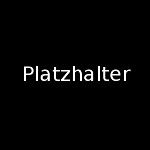
\includegraphics[scale=1.0]{spacer}
		\caption{Funktionsmodule der Anwendungssoftware}
		\label{fig.modules}
	\end{center}
	%\vspace*{-8mm}
\end{figure}

Das \mLocalization bestimmt und überwacht die aktuelle Position des Kamera-Projektor-Systems. Es ermittelt die initiale Position mittels globaler Lokalisation auf Basis der vom \mMapserver zur Verfügung gestellten Karte. Als weitere Eingangsgröße verwendet es die Odometriedaten, welche vom \mEkf zur Verfügung gestellt werden um Veränderungen in der Position während der Bedienung zu erkennen und die Positionsdaten dementsprechend zu aktualisieren. Das \mEkf selbst verwendet und filtert dabei die visuellen Odometriedaten des \mFovis und die Lagedaten des \mImu \red[TODO Moduls] um die kombinierten Odometriedaten zu bestimmen.\\
Diese so vom \mLocalization bestimmten Positionsdaten werden dann dem \mTransformation übermittelt, welches alle Koordinatentransformationen zwischen der ermittelten Kameraposition, dem Projektor und den relevanten Objekten der Umgebung berechnet. Diese Berechnungen werden dann vom \mVisualization verwendet, um ein Abbild der aktuellen Projektorsicht innerhalb der 3D Umgebung zu erstellen. Diese Ansicht wird dem Benutzer anschließend sowohl über die Benutzeroberfläche durch das \mGui als auch über die Projektion durch das \mProjection dargestellt. Das \mInteraction erkennt vom Benutzer durchgeführte Gesten oder Bewegungen, über welche er auf Basis der projizierten Daten mit der Modellumgebung interagiert. Die Steuerungsbefehle werden dann über das \mTransformation an das \mVisualization übertragen, wo diese interpretiert werden und in Form von Modifikationen der Modellumgebung umgesetzt werden.\\
Die jeweilige spezifische Realisierung der Module wird in den folgenden Kapiteln näher spezifiziert.
